 \documentclass[12pt,english]{article}
\usepackage[utf8]{inputenc}
\markright{Pearse et al.\hfill Assessing the Effects Imputation on ED Values\hfill}
\usepackage{geometry}
\geometry{verbose,letterpaper,tmargin=2.54cm,bmargin=2.54cm,lmargin=2.54cm,rmargin=2.54cm}
%\geometry{verbose,letterpaper,tmargin=.1cm,bmargin=.1cm,lmargin=.1cm,rmargin=.1cm}
\usepackage{graphicx}
\DeclareGraphicsExtensions{.pdf,.png,.jpg}
\usepackage{amssymb,amsmath}
\usepackage{epstopdf}
\usepackage{tocbibind}
\usepackage[toc,page]{appendix}
\usepackage{supertabular}
\DeclareGraphicsRule{.tif}{png}{.png}{`convert #1 `dirname #1`/`basename #1 .tif`.png}
\usepackage{url}
\usepackage{subcaption}
\usepackage{caption}
\usepackage[super]{nth}
\usepackage{lineno} \linenumbers
\usepackage[doublespacing]{setspace}
\usepackage[parfill]{parskip}
\setlength{\parindent}{0pt}
\usepackage[citestyle=authoryear,bibstyle=authoryear,sorting=nyt,maxcitenames=2,maxbibnames=10,minbibnames=6,doi=false,url=false,isbn=false,firstinits=true,uniquename=false,uniquelist=false]{biblatex}
\bibliography{edge_sims}
\renewbibmacro*{name:andothers}{% Based on name:andothers from biblatex.def
  \ifboolexpr{
    test {\ifnumequal{\value{listcount}}{\value{liststop}}}
    and
    test \ifmorenames
  }
    {\ifnumgreater{\value{liststop}}{1}
       {\finalandcomma}
       {}%
     \andothersdelim\bibstring[]{andothers}}
    {}}
\renewcommand*{\finalnamedelim}{%
  \ifnumgreater{\value{liststop}}{2}{\finalandcomma}{}%
  \addspace\&\space}
\renewbibmacro{in:}{}
\AtEveryBibitem{%
  \clearfield{day}%
  \clearfield{month}%
  \clearfield{endday}%
  \clearfield{endmonth}%
}
\DeclareFieldFormat[article]{citetitle}{#1}
\DeclareFieldFormat[article]{title}{#1}
\DeclareFieldFormat[article]{pages}{#1}
\DeclareNameAlias{sortname}{last-first}

\usepackage{changes}
\setdeletedmarkup{\textcolor{red}{\sout{#1}}}

\begin{document}
\setlength{\parindent}{0pt}
\section*{Title page}

\textbf{Article title}: Assessing the Effects Imputation on ED Values

\textbf{Running head}: Assessing the Effects Imputation on ED Values

\textbf{Authors:} K.\ Bodie Weedop$^{1}$, William D.\ Pearse$^{1}$\

$^1$ Department of Biology \& Ecology Center, Utah State University,
5305 Old Main Hill, Logan UT, 84322

$^*$To whom correspondence should be addressed:
\url{will.pearse@usu.edu} and \url{bodie.weedop@aggiemail.usu.edu}

\textbf{Word-count}: 5680 (abstract, main text, acknowledgements, and
  references)

\clearpage
\section*{Abstract}


\textbf{Keywords}: 

\clearpage
\section*{Introduction}
Evidence from the fossil record and present-day studies argue we are in the
midst of, or entering, a sixth mass extinction \autocite{Barnosky2011,
Ceballos2015}, such that more species than ever are declining and/or in danger
of extinction across a range of environments \autocite{Wake2008,Thomas2004}.
Habitat destruction \autocite{Brooks2002}, invasive species
\autocite{Molnar2008}, climate change \autocite{Pounds2006}, and disease
\autocite{Lips2006} are some of the leading causes of species declines
globally. Conservation biologists seek to overcome these declines and their
detrimental effects on species populations. Even still, researchers and
conservationists are confronted with ``Noah's Ark problem''
\autocite{Weitzman1998}, or an unfortunate reality of insufficient, finite
resources to confront the increasing amount of species requiring conservation
effort.

Conservation triage has provided an efficient decision making process for
allocating finite resources to obtain the greatest return
\autocite{Bottrill2008}. One of these triage strategies which have been
introduced and used most widely is EDGE \autocite{Isaac2007}. This method
prioritizes species according to two metrics: evolutionary distinctiveness (ED)
and global endangerment (GE). ED measures relative contributions to phylogenetic
diversity made by each species within a particular clade \autocite{Isaac2007}.
Such contributions are assessed by quantifying the amount of branch length which
is unique to each species within the overall phylogeny. GE values are assessed
by assigning numerical values to each of the World Conservation Union (IUCN) Red
List Categories. As species become increasingly threatened and are placed into
more concerning categories (e.g. from Vulnerable to Endangered), the GE
numerical value increases. Increases in either ED or GE place a particular
species at a higher priority for conservation effort.

In the event of missing DNA or trait data, species are often difficult or not
able to be placed onto a phylogeny. Regardless of such uncertainty and missing
data for certain species, it is understandable that reseachers may want to
include those species while making conservation priorities. However, if we are
using a quantitative method for prioritizing species, we should remain
consistent even when uncertainty arises. To our knowledge, a proper and
efficient method for prioritizing species where there is missing data is still
untested. This issue pertains mainly to the calculation of ED rather than GE. In
terms of GE, the IUCN has a strategy for assigning Red Listing values to species
which we have little information and are considered Data Deficient (DD). IUCN
and other conservation organizations support focus on DD species just the same
as Critically Endangered and Endangered species to ensure consistency
\autocite{Rodrigues2006}. The major area of uncertainty in phylogenetic
prioritisation is phylogenetic data. In the past, missing species data and
poorly resolved trees have been addressed using imputation
\autocite{Collen2011, Isaac2012, Jetz2014}. However, to our knowledge, there has
been no systematic investigation of the efficacy of such method, both in
terms of the accuracy with which imputed ED values are estimated, and the effect
on other known species’ scores. Indeed, it is unclear whether any significant
information on ED is gained by imputing species which cannot be placed on the
phylogeny. It is also not well understood how simply excluding missing species,
compared to performing imputation, would effect ED values. It may be that
excluding missing species may be less intrusive than imputation. In searching
for a solution for missing species, we may be negatively affecting correct ED
values and disrupting EDGE rankings in the process. As the desire to use ED and
phylogenies for conservation triage grows, the importance of such tests and a
consensus on how to resolve cases of phylogenetic uncertainty becomes more
urgent.

Here, we assess and compare the impact that missing species versus phylogenetic
imputation has upon ED values. In doing so, we hope to understand the effect
that both methods have on ED values and offer a viable solution for dealing with
missing data species. In order to do so we simulated missing species and removed
them from trees in two ways: randomly and in a phylogenetically biased manner.
Additionally, we tested how ED values were affected by resolving and imputing
polytomies of varying sizes on a phylogeny. Through these investigations we
found that 1) missing a proportion of species, at random and in a
phylogenetically biased manner, has an effect on correctly assigning ED values
2) imputing species within a clade negatively affects the informative value of
ED for other species in the same clade.  

\section*{Methods}
We attempted to demonstrate the effects of removing or imputing
species which cannot be placed onto a phylogeny. While assessing the
impact of dropping species and phylogenetic imputations, we were
primarily focused on ED values. In testing the effects on these
values, we remain focused upon ED as a single variable. We exclude GE
because it would only add complexity while not providing any
additional information to our particular investigation.

In each test, we simulated 100 phylogenetic trees and manipulated each
tree’s tips or clade. All simulations, calculations, and analyses were
performed using R (version 3.4.0). Original and manipulated trees were
simulated under a pure-birth Yule model using the sim.bdtree function
‘geiger’ R package \autocite{Harmon2007}. This particular model was
chosen to maintain simplicity. Results from this simple model should
be applicable to other more complex scenarios. Also, to reduce
uncertainty, we used the same model throughout each of the
simulations. In reality, we would be estimating the parameters of the
model which the phylogeny is built upon. The function ed.calc within
the R package ‘caper’ was used to calculate ED values for each tree
\autocite{Orme2013}.

We assessed the impact that removing missing species has upon ED
values using the correlation of all ED values for the tips remaining
within both trees. To evaluate the effect that imputation has upon ED
values, we calculated ED for all tips in both the original and
manipulated trees while excluding the focal clade where imputation has
occurred. These ED values were compared using a
correlation. Additionally, we did the same calculations and comparison
using only the original focal clade and its’ simulated replacement. If
missing species have no effect upon ED values, we expect a high,
positive correlation coefficient between the original tree and its’
manipulated counterpart.

\subsection*{Assessing the impact of missing species on EDGE-listing}
If missing species has a negative effect on ED values, then the
correlation between the ED of the species in the original tree and the
same tree with a fraction of tips removed in some manner should be
significantly different from 1. To investigate the degree of this
effect, we removed tips from simulated trees (Number of taxa = 64,
128, 256, 512, 1024, 2048, 4096) at random and by phylogenetic
clusters. To assess the effect under varying amounts of uncertainty,
fractions of tips dropped ranged from 0 to 0.99 of total tree tips. 
To compare ED values before and after species are removed fom the 
phylogeny, we correlate both ED values of only the species 
which remain in the phylogeny. 

Missing species at random was simulated by selecting species at random
without replacing, and removing those species from the tree. This
randomization had no regard for phylogenetic structure. Missing
species related by some character trait was tested by simulating
character trait values for each tip. These simulations were all
performed under a constant rate Brownian-motion model (par = 0.5,
starting root value = 1). Tips were dropped if their character trait
values place them into the upper quantile which had been selected to
be dropped. More specifically, if the fraction to be dropped was 0.1,
species within the 90th quantile of character trait values are
dropped. This is equivalent to Felsenstein’s threshold model
\autocite{Felsenstein2004}.

\subsection*{Assessing the impact of phylogenetic imputations}
We tested the impact of imputing missing species onto a clade of a
particular size (sizes 3 through 32) which originated
from a tree of a particular size (Number of taxa = 64, 128, 256, 512,
1024). To simulate the effect that phylogenetic imputation has upon
these simulated trees, we randomly chose clades within each tree and
treated it as a polytomy to be resolved. The clade selected was
removed from the original tree and a new separate tree of the same
size was simulated under the pure-birth model used before and placed
back where the original clade was removed. By doing this , we
replicated the process of imputation of a clade which has been
resolved. To ensure that this is representative of cases where
imputation is used, 100 repetitions of this simulation were performed
across different parameter settings.

\section*{Results}
\subsection*{Assessing the impact of missing species on EDGE-listing}

Our results demonstrate that the comparison between ED values before and after
species were removed was negatively affected by the fraction of species removed
in both treatments (Table 1). Similar but slightly different effects are seen
when dropping species at random and in clustered manner (Fig.
\ref{randomVsClustered}). Interestingly, the rate at which ED values deviate
from their true value is increased with species missing at random. 

\begin{figure}[!ht]
  \center
  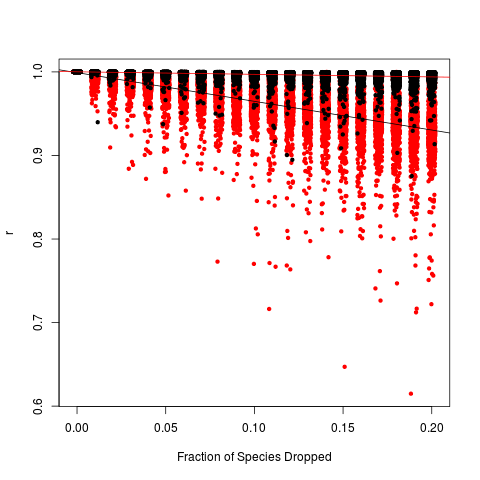
\includegraphics[width=.5\textwidth]{randomVsCluster.png}
  \caption{\textbf{R-values plotted against the fraction of species dropped at
  random versus clustered manner.} The color of data points denote whether
  species were dropped at random (orange; n = 100) or in clustered manner
  (grey; n = 100). The regression lines are demonstrating the relationship when
  species are dropped at random (red) and in a clustered manner (clustered). The
  correlations represent a comparison of the ED values (before and after
  species are dropped) of species which remain on the on the phylogeny after
  other species are dropped. 
  }
  \label{randomVsClustered}
\end{figure}

\begin{table}[ht]
  \centering
  \begin{tabular}{rrrrr}
    \hline
   & Estimate & Std. Error & t value & Pr($>$$|$t$|$) \\
    \hline
  (Intercept) & 1.0315 & 0.0013 & 821.39 & $<$0.0001 \\
    Fraction of Species Dropped & -0.4696 & 0.0020 & -233.16 & $<$0.0001 \\
    Random Treatment & 0.0630 & 0.0018 & 35.47 & $<$0.0001 \\
    Number of Species Overall & 0.0000 & 0.0000 & 7.89 & $<$0.0001 \\
    Fraction of Species Dropped:Random Treatment & -0.2774 & 0.0028 & -97.45 & $<$0.0001 \\
    Random Treatment:Number of Species Overall & 0.0000 & 0.0000 & -4.38 & $<$0.0001 \\
     \hline
     \hline
  \end{tabular}
  \caption*{\textbf{Table 1: ANCOVA model summary describing the effect of
  dropping species on remaining species ED Values.} The fraction of species
  dropped significantly affects the the remaining ED values. Dropping the
  fraction both at random and in clustered manner both have negative effects on
  the remaining ED values ($F_{139696, 5}$ = 40350, $R^{2}$ = 0.5908,
  p$<$0.0001).}
  \end{table}

\subsection*{Assessing the impact of phylogenetic imputations}

ED values for the full tree while excluding the focal clade remain at 1 and
unaffected. However, ED values for the imputed clades are significantly
affected by the use of imputation. As the size of the focal clade increases,
the informative value of the ED values within the clade decreases (Fig.
\ref{imputationTrend}). However, even when imputing smaller clades, ED values
did not regularly reflect the true ED values (Table 2). Our analysis
demonstrates that measures of the original phylogeny such as phylogentic
diversity (PD), lambda, Colless' Index, skew, and kurtosis do not provide any
indication that imputation would negatively affect ED values (Appendix A).
Additionally, just as imputed ED values did not reflect true ED values, the
rankings of species within the focal clade were altered significantly (Fig.
\ref{rankingError}). Our model suggests that with increases in the size of the
imputed clade and overall number of species, species within the clade are
ranked farther from their true ranking (Table 3). More specifically, our model
suggests that by imputing a clade of three species within a phylogeny of 128
species, the species within the clade would be 60 rankings from their true rank
on average. ED values outside of the focal clade were not affected by
imputation. While ED values within the focal clades were affected exclusively
by imputation, a notable error rate in ranking crucial species correctly is
present (Appendix B).

\begin{figure}[!ht]
  \center
  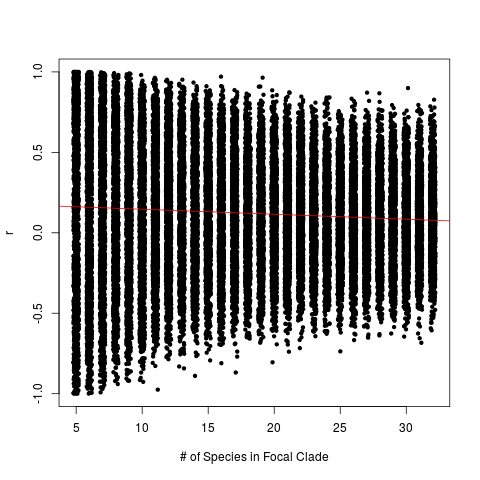
\includegraphics[width=.5\textwidth]{edModel.png}
  \caption{\textbf{R-values plotted against the number of species at focal
  clade.} Each data point denotes a correlative comparison between ED values
  within the focal clades where imputation has occurred. The regression line
  (red) and trend even closer to zero demonstrates the decrease in informative
  value of the imputed ED values. This is reinforced by the visual narrowing of
  r-values around zero.}
  \label{imputationTrend}
\end{figure}

\begin{table}[ht] 
\centering
\begin{tabular}{rrrrr}
  \hline
  & Estimate & Std. Error & t value & Pr($>$$|$t$|$) \\
   \hline
 (Intercept) & 0.1852 & 0.0533 & 3.47 & 0.0005 \\
   Size of Focal Clade & -0.0034 & 0.0002 & -16.56 & 0.0000 \\
   Size of Phylogeny & -0.0001 & 0.0001 & -0.41 & 0.6855 \\
   PD & 0.0001 & 0.0001 & 0.37 & 0.7108 \\
   Lambda & -0.0012 & 0.0524 & -0.02 & 0.9812 \\
   Colless' Index & 0.0016 & 0.0022 & 0.72 & 0.4687 \\
   Skew & 0.0043 & 0.0088 & 0.48 & 0.6288 \\
   Kurtosis & -0.0005 & 0.0009 & -0.63 & 0.5269 \\
   \hline
   \hline
\end{tabular}
\caption*{\textbf{Table 2: Effect of Clade Size on Imputed ED Values.} The
intercept describes that the correlation between the true and imputed values
begins quite low. As the clade size increases, this correlation only tends
toward zero. The total number of species in the full phylogeny along with
measures of the true phylogenetic diversity, lambda, Colless' Index, skew, and
kurtosis show no significant effect. ($F_{47992, 7}$ = 39.57, $R^{2}$ = 0.006,
p$<$0.0001).}
\end{table}

\begin{figure}[!ht]
  \center
  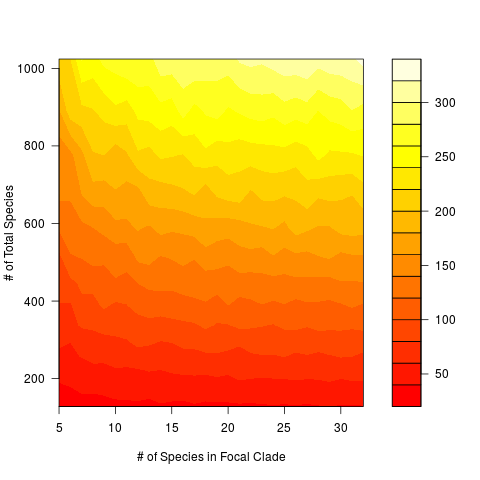
\includegraphics[width=.5\textwidth]{rankingError.png}
  \caption{\textbf{Mean ranking error of species within the focal clade.} The 
  gradient on the right demonstrates average number of posistions within the 
  full ranking that focal clade species shifted from their true rank.
  While controlling for the size of the full phylogeny and focal clade, species 
  within the focal clade were, on average, ranked far from the true rank. }
  \label{rankingError}
\end{figure}

\begin{table}[ht]
  \centering
  \begin{tabular}{rrrrr}
    \hline
   & Estimate & Std. Error & t value & Pr($>$$|$t$|$) \\
    \hline
  (Intercept) & -1.6344 & 0.0332 & -49.29 & 0.0001 \\
    Size of Focal Clade & 0.0900 & 0.0010 & 91.22 & 0.0001 \\
    Size of Phylogeny & 0.5179 & 0.0013 & 383.99 & 0.0001 \\
     \hline
     \hline
  \end{tabular}
  \caption*{\textbf{Table 3: Effect of Clade Size and Total Species on Ranking
  Error.} Model demonstrating the relationship between focal clade species
  ranking error and the size of imputed clade and overall phylogeny. Square-root
  transformations have been applied to both ranking error and size of phylogeny.
  Significant increases ranking error are seen when increasing sizes of both the
  imputed clade and phylogeny ($F_{47997, 2}$ = 77890, $R^{2}$ = 0.7644,
  p$<$0.0001).}
  \end{table}

\clearpage
\section*{Discussion}
Phylogenetic uncertainty and missing species are complications commonly
encountered when applying ED for prioritization \autocite{Isaac2007}. The aims
of our investigation were to (1 determine how removing missing species from a
phylogeny affects ED values for the remaining species and (2 demonstrate how
imputation affects ED values of species where imputation is performed. Our
results demonstrate that (1 missing a proportion of overall species both at
random and in a phylogenetic-biased manner have different yet significant
affects on remaining ED values throughout the tree and 2) imputation does not
recover the ED value or ED rank of an imputed species.

Missing species and poor phylogenetic resolution have been identified as causes
of uncertainty when calculating ED \autocite{Isaac2007}. Prior to our
investigation, we could not find any assessment of how missing species might
affect ED values of species which are not missing. Our results demonstrate that
missing species at random or in a phylogenetically-biased manner can have
different effects on ED values \ref{randomVsClustered}. Both manners of missing
species cause ED values of species easily placed on the phylogeny to stray from
their true values (Table 1). Missing species at random  However, the manner
(either randomly or phylogenetically-patterned) in which species are missing
from the phylogeny is, to our knowledge, not normally investigated when deciding
how to address them. In light of our results, this should be a concern when
deciding how to move forward with missing species. We realize that we have
provided just two ways in which species could be missing from a phylogeny and
there are more that could occur. Missing species could be biased by some
phylogenetic pattern other than Brownian motion evolution. Nevertheless, our
investigation shows that missing species cause ED values of species remaining in
the phylogeny to deviate from the true value.

In the past, we have included missing species into the EDGE framework using
different methods. Collen et al. assigned the mean ED score of presumed
congeneric species to the missing species \citeyear{Collen2011}. More
frequently, missing species and poorly resolved clades have been dealt with by
imputing the missing species and assigning all the species of the resolved
clade the mean ED value obtained from all possible or numerous resolutions of
the clade \autocite{Isaac2007; Isaac2012}. This method has been adapted by
others and applied where there were large percentages (~30\%) of species
missing \autocite{Jetz2014}. While imputation does include missing species,
research has shown imputed phylogenetic data leads to biases in some ensuing
analyses \autocite{Rabosky2014}. When considering the analysis of ED, our
results show that imputation does not recover true ED values nor ED rank of
missing species \ref{imputationTrend; rankingError}. Additionally, as the size
of the imputed clade increases, ED values within the clade stray, on average,
further from their true values. Even though we are including missing species
into calculating ED, we are not obtaining accurate information about those
species. While being uninformative, these ED values would lead to
mispriortizing species based on our results \ref{rankingError}. Analyzing the
performance of imputation of a clade less than five species was not performed
due to limitations of statistical validity \autocite{Crawley2012}. Even so, our
results provide no indication that the effects of imputation seen in our
results would improve when applied at smaller clades.

Combining the previous arguments provides an interesting case of when imputation
could be useful. Both random and phylogenetically-patterned loss of species
affect ED values throughout the tree. However, we found that ED values of
non-missing species remain relatively constant under imputation. Therefore,
imputation provides an interesting solution to missing species biasing ED
values of non-missing species. We have shown that imputing missing species would
not provide accurate ED values for missing species. However, it would provide a
method of avoiding the loss of species affecting ED values throughout the
remainder of the tree. Basing conservation priorities upon the ED values of
imputed species would lead to inaccurate prioritization. Nevertheless,
imputation may be useful to stop missing species from biasing species easily
placed on the phylogeny.

We acknowledge that a Yule model of evolution is a simple model and more complex
models may be present in empirical data. While we do not have empirical data,
our simulations are performed under the same evolutionary model and therefore
able to generalize for more complicated cases which might be seen in empirical
data. However, our results demonstrate that even under a simple model imputing
species lead to a misrepresentation of true ED values. Also, we have not been
given any implication through this investigation that a more complex model would
give any different results. Nomrally, imputation is averaged across all numerous
trees to get the closest estimate of true ED values. However, imputed trees
still deviate from the true trees and therefore the average would also be far
from the true average.

Given these results, we have developed several guidelines for how missing
species should be dealt with and when imputation might be appropriate when
calculating EDGE. In the event of missing species, we should be investigating
the amount of species that are missing and consider whether imputation is
necessary. For some context, in our analysis we found that if 30\% of species
are missing at random or in a phylogenetic-biased manner from the phylogeny,
respectively, ~80\% and ~89\% of the remaining ED values remained accurate.
Therefore if species are missing, we should verify that the amount of missing
species does not exceed a percentage which we have found to provide poor ED
values for remaining species. While below an acceptable percentage of missing
species, EDGE should be carried out without attempting to impute the
missing species. However, if a larger proportion of species are missing,
imputation may be used but with some caution. ED values for species easily
placed on the phylogeny are relatively unaffected and can be trusted when
setting conservation priorities. Nevertheless, ED values and ranks of species
which have been imputed should either be ignored or used cautiously within EDGE.
By following these guidelines we avoid biasing species which are easily placed
on the phylogeny even in the event that imputation is used.

\section*{Acknowledgments}

\clearpage
\printbibliography

\clearpage
\appendix
\section*{A. Effect of Measures of the True, Full Phylogenies}

\begin{figure}[!ht]
  \center
  
\includegraphics[width=.5\textwidth]{trueColless.png}
  \caption{\textbf{Effect of the True Colless Index of FullPhylogeny.}}
\end{figure}

\begin{figure}[!ht]
  \center
  
\includegraphics[width=.5\textwidth]{trueLambda.png}
  \caption{\textbf{Effect of the True Lambda of Full Phylogeny.}}
\end{figure}

\begin{figure}[!ht]
  \center
  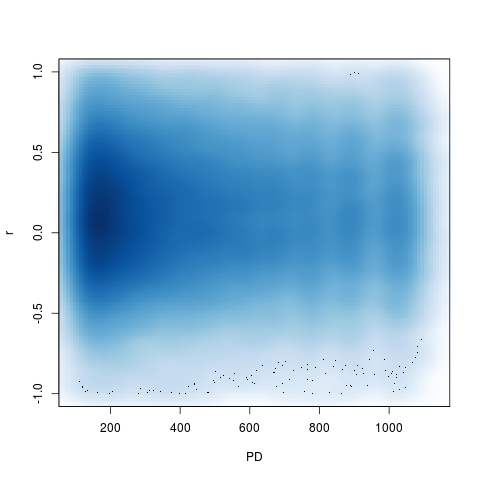
\includegraphics[width=.5\textwidth]{PD.png}
  \caption{\textbf{Effect of True PD of Full Phylogeny.}}
\end{figure}

\begin{figure}[!ht]
  \center
  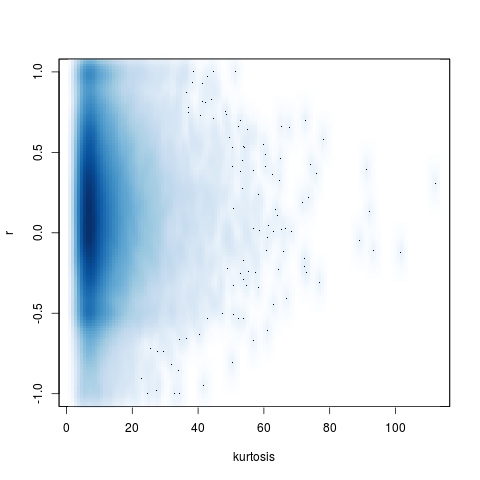
\includegraphics[width=.5\textwidth]{originalKurtosis.png}
  \caption{\textbf{Effect of the True Kurtosis of Full Phylogeny.}}
\end{figure}

\begin{figure}[!ht]
  \center
  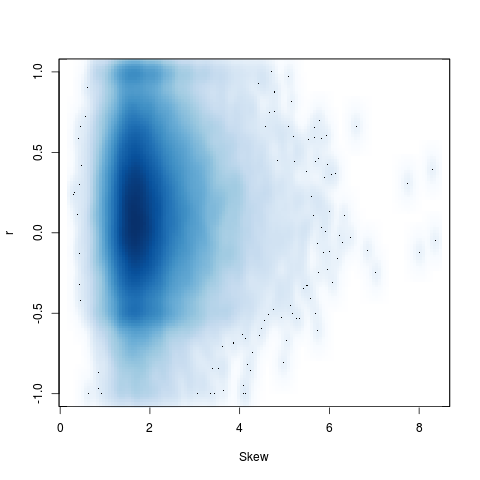
\includegraphics[width=.5\textwidth]{originalSkew.png}
  \caption{\textbf{Effect of the True Skew of Full Phylogeny.}}
\end{figure}

\clearpage
\clearpage
\section*{B. Error Rate in Top Rankings}

\begin{figure}[!ht]
  \center
  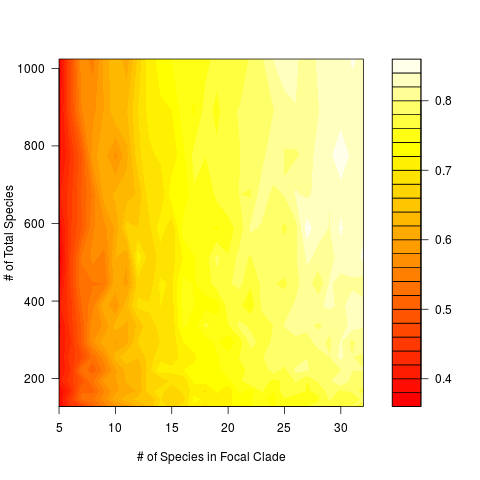
\includegraphics[width=.5\textwidth]{errorRate50.png}
  \caption{\textbf{Mean error rate in the ranking of top 50 species.}}
\end{figure}

\begin{figure}[!ht]
  \center
  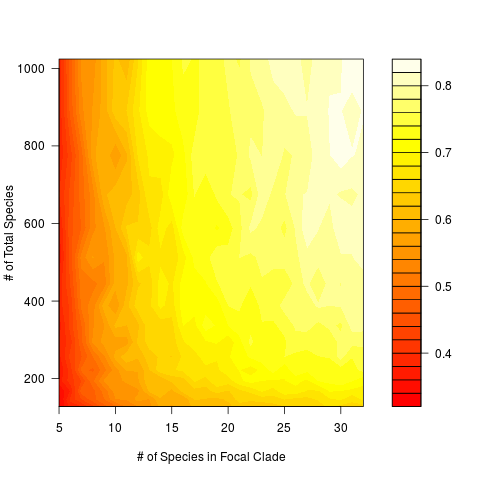
\includegraphics[width=.5\textwidth]{errorRate100.png}
  \caption{\textbf{Mean error rate in the ranking of top 100 species.} }
\end{figure}

\begin{figure}[!ht]
  \center
  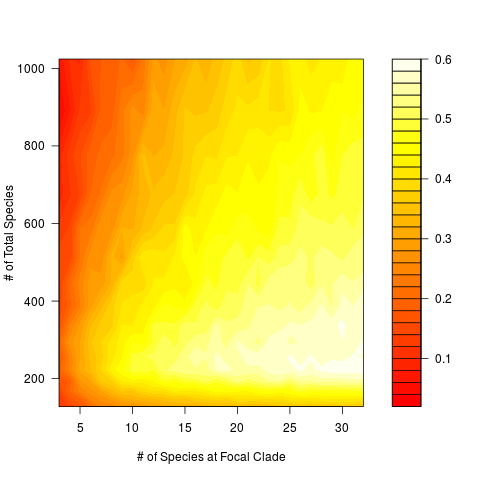
\includegraphics[width=.5\textwidth]{errorRate200.png}
  \caption{\textbf{Mean error rate in the ranking of top 200 species.} }
\end{figure}

\begin{figure}[!ht]
  \center
  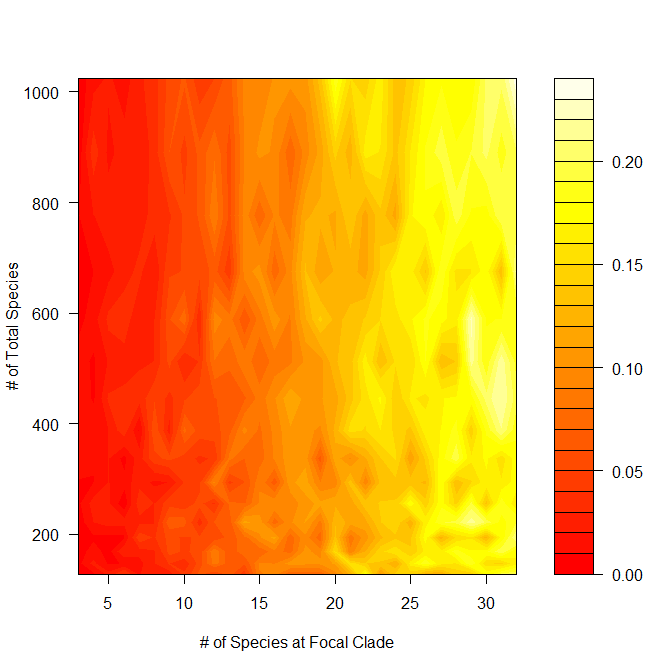
\includegraphics[width=.5\textwidth]{errorRate5pct.png}
  \caption{\textbf{Mean error rate in the ranking of top 5\% of species.} }
\end{figure}

\begin{figure}[!ht]
  \center
  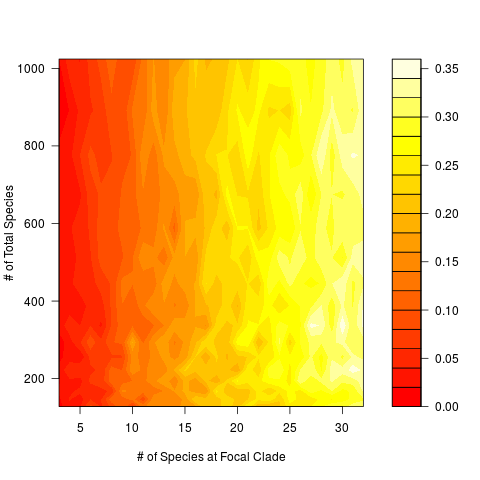
\includegraphics[width=.5\textwidth]{errorRate10pct.png}
  \caption{\textbf{Mean error rate in the ranking of top 10\% of species.} }
\end{figure}

\begin{figure}[!ht]
  \center
  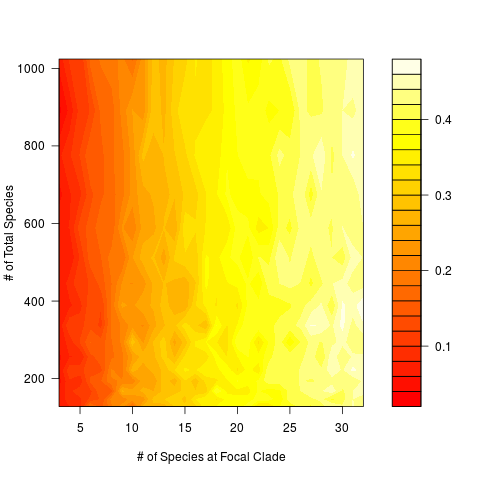
\includegraphics[width=.5\textwidth]{errorRate20pct.png}
  \caption{\textbf{Mean error rate in the ranking of top 20\% of species.}}
\end{figure}

\end{document}
%%% Local Variables:
%%% mode: latex
%%% TeX-master: t
%%% End: